%!TEX root = ../PhD_thesis__Lilian_Besson

% First chapter begins here
\chapter{Introduction}
\label{chapter:1}

\TODOL{Lundi soir : je dois encore relire le 1.1 pour les fautes d'orthographe (et les éventuels erreurs historiques) !}
\TODOL{Lundi soir : je dois encore terminer le 1.2 et être plus concis ?}
\TODOL{Je dois écrire le 1.3 en max 2 pages : j'ai déjà le plan, je dois développer}

\abstractStartChapter{}%
%
We start by presenting the context then the problems studied in this thesis.
We further announce the different directions we considered and the solutions we proposed.
We give an overview of our main contributions, alongside a list of publications written in the last three years.
%
The organization of this manuscript is detailed in a flow graph, which highlights that Chapters~\ref{chapter:4} to \ref{chapter:6} are partly independent, but they are all built upon the model and notations introduced on Chapter~\ref{chapter:2}.

\TODOL{J'enlève l'abstract et la minitoc dès que le chapitre est terminé !}

\minitocStartChapter{}

% Write miniTOC just after the title
\graphicspath{{2-Chapters/1-Chapter/Images/}}


% ----------------------------------------------------------------------------
\section{Context of this thesis}
\label{sec:1:problems}

% Where
\textbf{Where and when?}
%
This doctoral thesis started in October $2016$, and finished in October $2019$.
My research took place at the IETR laboratory in Rennes (France), in the SCEE team hosted on the Rennes campus of the engineering college CentraleSupélec.
In Rennes I was supervised by Professor Christophe Moy,
and I was also co-supervised by Doctor Emilie Kaufmann, whom I visited many times at Inria Lille Nord Europe in Lille (France).

\TODOL{Est-ce que je dois détailler plus ? Quel financement j'ai eu (CDSN), quels autres financements m'ont aidés ?}

% Main problem
\textbf{Main problems.}
%
At the root of the problems that motivates this thesis are the questions of global warming, and the increase of the world population.
% https://en.wikipedia.org/wiki/History_of_radio
During the last 150 years, mankind has developed a wide range of different communication technologies, and since the late $1890$s wireless communications between devices have been made possible, and more and more frequent in our lives.
With the avent of Internet of Things networks (IoT), billions of autonomous low-power devices are expected to be deployed world-wide, for a large range of different applications.
It is now well-known that with the current trend of population increase and with the energy crisis, any newly deployed technology should be cheap and energy efficient,
as well as adapted to serve a large number of people and devices.

That is why we are interested in this thesis about the possible applications of embedding a certain kind of Machine Learning algorithms (MAB algorithms),
directly into the future IoT devices, in order to improve their battery life and reduce the energy cost of IoT networks, by optimizing the wireless communication thanks to embedded decentralized decision making.


\paragraph{From old TV to the IoT standards.}
%
Historically, three families of wireless communication systems have been deployed: first, centralized broadcasting (\eg, old TV), then centralized bi-directional systems (\eg, 4G or WiFi), and nowadays decentralized broadcasting for the Internet of Things networks (IoT).

% Central broadcasting
Starting from FM radio music and news, then old black-and-white TV and color TV, the first systems were purely made for centralized broadcasting of information. In a large area, one antenna well located emits continuously in a fixed Radio Frequency (RF) band, and many devices can listen to this RF traffic and decode it, for instance to listen to music.
Different standards have been developed, and some of them are still in use today, and their nature requires a central authority that allocates RF bands to different usages (\eg, TV channels etc).
For example, in the city of Cesson-Sévigné where the campus of CentraleSupélec is located, a high RF tower emits on many standards, and in particular the \SI{92.3}{\mega\hertz} band is allocated to a French classical music radio (\emph{Radio Classique}).
Broadcast-based systems are not only used for TV or radio,
and for instance two other famous and world-wide deployed examples are the long-range Global Positioning System (GPS), and short-range infrared remote controllers.

% Two ways communications
However, this kind of mono-directional wireless communications were soon found to not be satisfactory for many applications, and thus bi-directional standards were defined from the $1910$s.
First developed by and for the military, and the navy (\eg, the Titanic sent the first SOS signal over radio in $1912$),
such applications have reached general public usage since the $1950$s.
The greatest achievement of this long-running R\&D domain was the avent of mobile telephony in the $1990$s, which has continued to be more and more present in people lives in the richer countries in the world, with the booming of cellphones since the $2000$s and smartphones since the $2010$s.
In most systems, there is still an antenna in charge of a large area (or cell), and many devices are able to receive and transmit data to the antenna.
Nowadays, the most well-known systems include WiFi, and systems deployed for mobile phone communications, with a long list of standards from 1G, 2G, 3G, 4G and now 5G, still in development in $2019$.
Even if both systems initially differed in usage, as 1G was designed to exchange only voice, and WiFi to link wireless devices at home to an Internet-connected box, they are conceptually very close.
As the systems are cellular, any device knows the antenna (or base station) it is associated with, and the bi-directional nature of their exchanges makes a centralized control possible.
In order to optimize the efficiency of the network, the base station is equipped with decision making algorithms that affects the devices in the cell to the available resources (time slots, RF bands, power etc).
To be able to communicate with the base station without interfering with each others, such affectation should be orthogonal, and led to systems based on Time Division Multiple Access (TDMA) and Frequency Division Multiple Access (FDMA), or Non-Orthogonal techniques only started to emerge recently (\eg, NOMA).
Traditionally, the base station aimed only at maximizing the Quality of Service (QoS), that englobes the data rate, latency, availability and other measures of performance of the wireless communications to and from the devices.
More recently, green radio has emerged as a solution to the tradeoff between maximizing QoS while minimizing the power consumption of base stations and devices.

% The opposite: decentralized broadcasting, and the age of IoT
Finally, a third kind of systems are of the opposite kind, and can be designed as decentralized broadcasting: an antenna is still in charge of many devices, but such devices can only send up-link packets, and the only down-link data they can receive are short acknowledgements sent from the base-station to indicate success or failure of an up-link packet.
This family of wireless systems are referred to as Internet of Things,
and a typical example of application is for sensor networks.\\
\indent
For the future development of smart grids, smart cities, smart homes, or smart agriculture, sensor networks are promised to be widely deployed.
Two examples of future applications that are already in deployment, in France or other countries, are connected buildings and connected agriculture.
For buildings, the main goal is to reduce the cost of heating empty buildings and use temperature sensor networks to get accurate and regular data about the temperature in each room and each floor, and let the centralized heat control optimize its cost and energy consumption.
For agriculture, one example can be to equipped every cow (in large farms) with a sensors that emits biological information, such as body temperature or stress level etc, in order to optimize the time of milking and monitors the health of the animals.\\
%
% OK commencer par un paragraphe qui explique qu'on étudie les télécom dans le but de les rendre automatiquement plus efficace, plus verte, plus adaptative
\indent
This third kind of wireless systems are characterized by their decentralized nature: due to the really limited information that the base station can send to the devices, it is no longer possible to optimize the efficiency of the network from the centralized point-of-view of the base station.
In the present and future IoT networks, many devices of heterogenous nature are using the same antenna for many different applications.
A common hypothesis is that such IoT devices have a strong constraint on their power consumption, as most of them will be deployed without a direct power access and will use a battery, which duration should be maximized (typically more than 10 years).
Another common constraint for IoT devices is their low duty cycle, as most applications target one to a few messages sent by day, in strike opposition to the high data-rate pursued for centralized systems such as 4G/5G and WiFi.
%
Many different standards for IoT networks have been proposed,
and they consist in a specification for both the \emph{PHY}sical
and the Medium Access Control (\emph{MAC}) layer.
To quote some examples of standards, ZigBee, Z-Wave or Bluetooth are targeting for short-range communications, while LoRaWAN, SIGFOX, Ingenu or Weightless are designed for long-range communications.
We refer to the survey \cite{Centenaro16} for more details, and references in \cite{Azari18} or our recent article \cite{MoyBesson2019}.

% OK commencer par décrire ce sur quoi porte la thèse, en deux phrases qui réduisent le cadre


\section{Cognitive Radio and Multi-Armed Bandits}

In this thesis, we study Internet of Things networks, and these two constraints of low power consumption (or long battery life) and low duty cycle are essential.
More precisely, we study the possible interconnections between \textbf{Machine Learning} and \textbf{Cognitive Radio} applied for IoT networks.
Let us define and detail both concepts.

% This thesis studies the possible applications of a certain kind of Machine Learning algorithms, Multi-Armed Bandits, to a certain kind of Telecommunications, Cognitive Radio and Internet of Things of Networks.


\paragraph{From Machine Learning to Multi-Armed Bandits.}
%
We can narrow down the first field of study of this thesis, steps by steps.
Starting from the general concept of Machine Learning (ML), we focused our interest to statistical learning, then sequential learning, then Reinforcement Learning (RL), then RL with limited feedback and finally to Multi-Armed Bandits (MAB) learning.
As illustrated in Figure~\ref{fig:1:MainTypesOfMachineLearning}, there are other types of ML, that we do not focus on in this thesis.
The reference book on RL is \cite{SuttonBarto2018}, so let us quote the definition of RL given by Richard Sutton and Andrew Barto:
\emph{``Reinforcement learning is learning what to do -— how to map situations to actions -— so
as to maximize a numerical reward signal. The learner is not told which actions to
take, but instead must discover which actions yield the most reward by trying them''}.
% - apprentissage statistique (machine learning) > séquentiel > par renforcement > information partielle (bandits)

% \begin{figure}[h!]
%     \centering
%     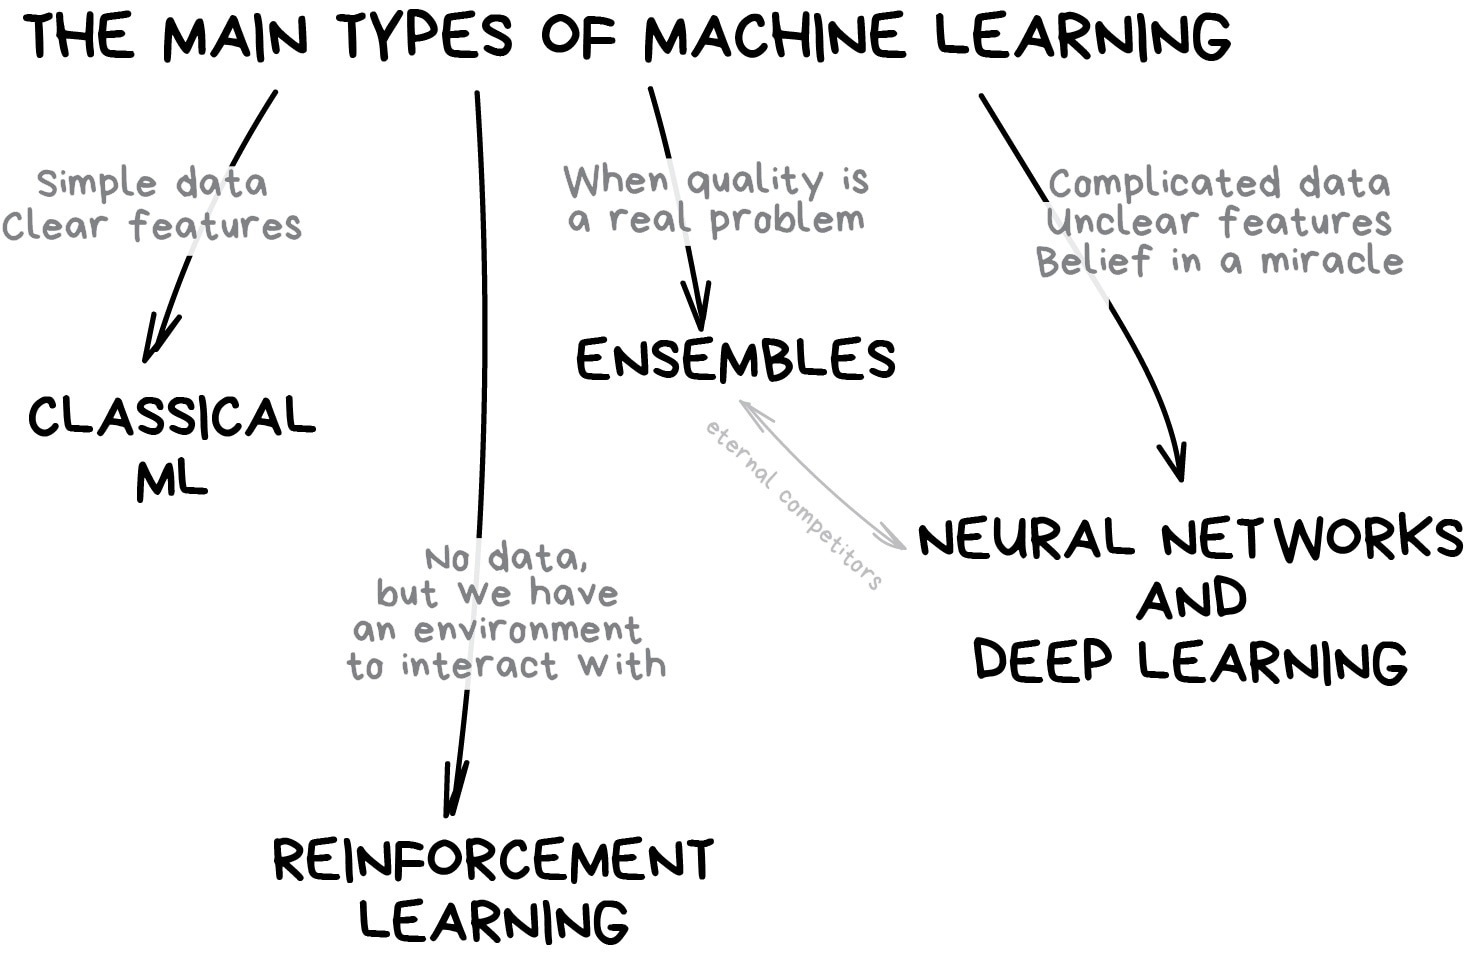
\includegraphics[width=0.45\textwidth]{Illustration_of_Machine_Learning_and_Reinforcement_Learning.jpg}
% \caption{Main types of Machine Learning, \copyright{} from \href{https://vas3k.com/blog/machine_learning/}{\texttt{VAS3k.com/blog/machine\_learning}}.}
% \label{fig:1:MainTypesOfMachineLearning2}
% \end{figure}

% Modified from the https://draw.io/ map from
% https://github.com/trekhleb/homemade-machine-learning/blob/master/images/machine-learning-map.xml
\begin{figure}[h!]
    \centering
    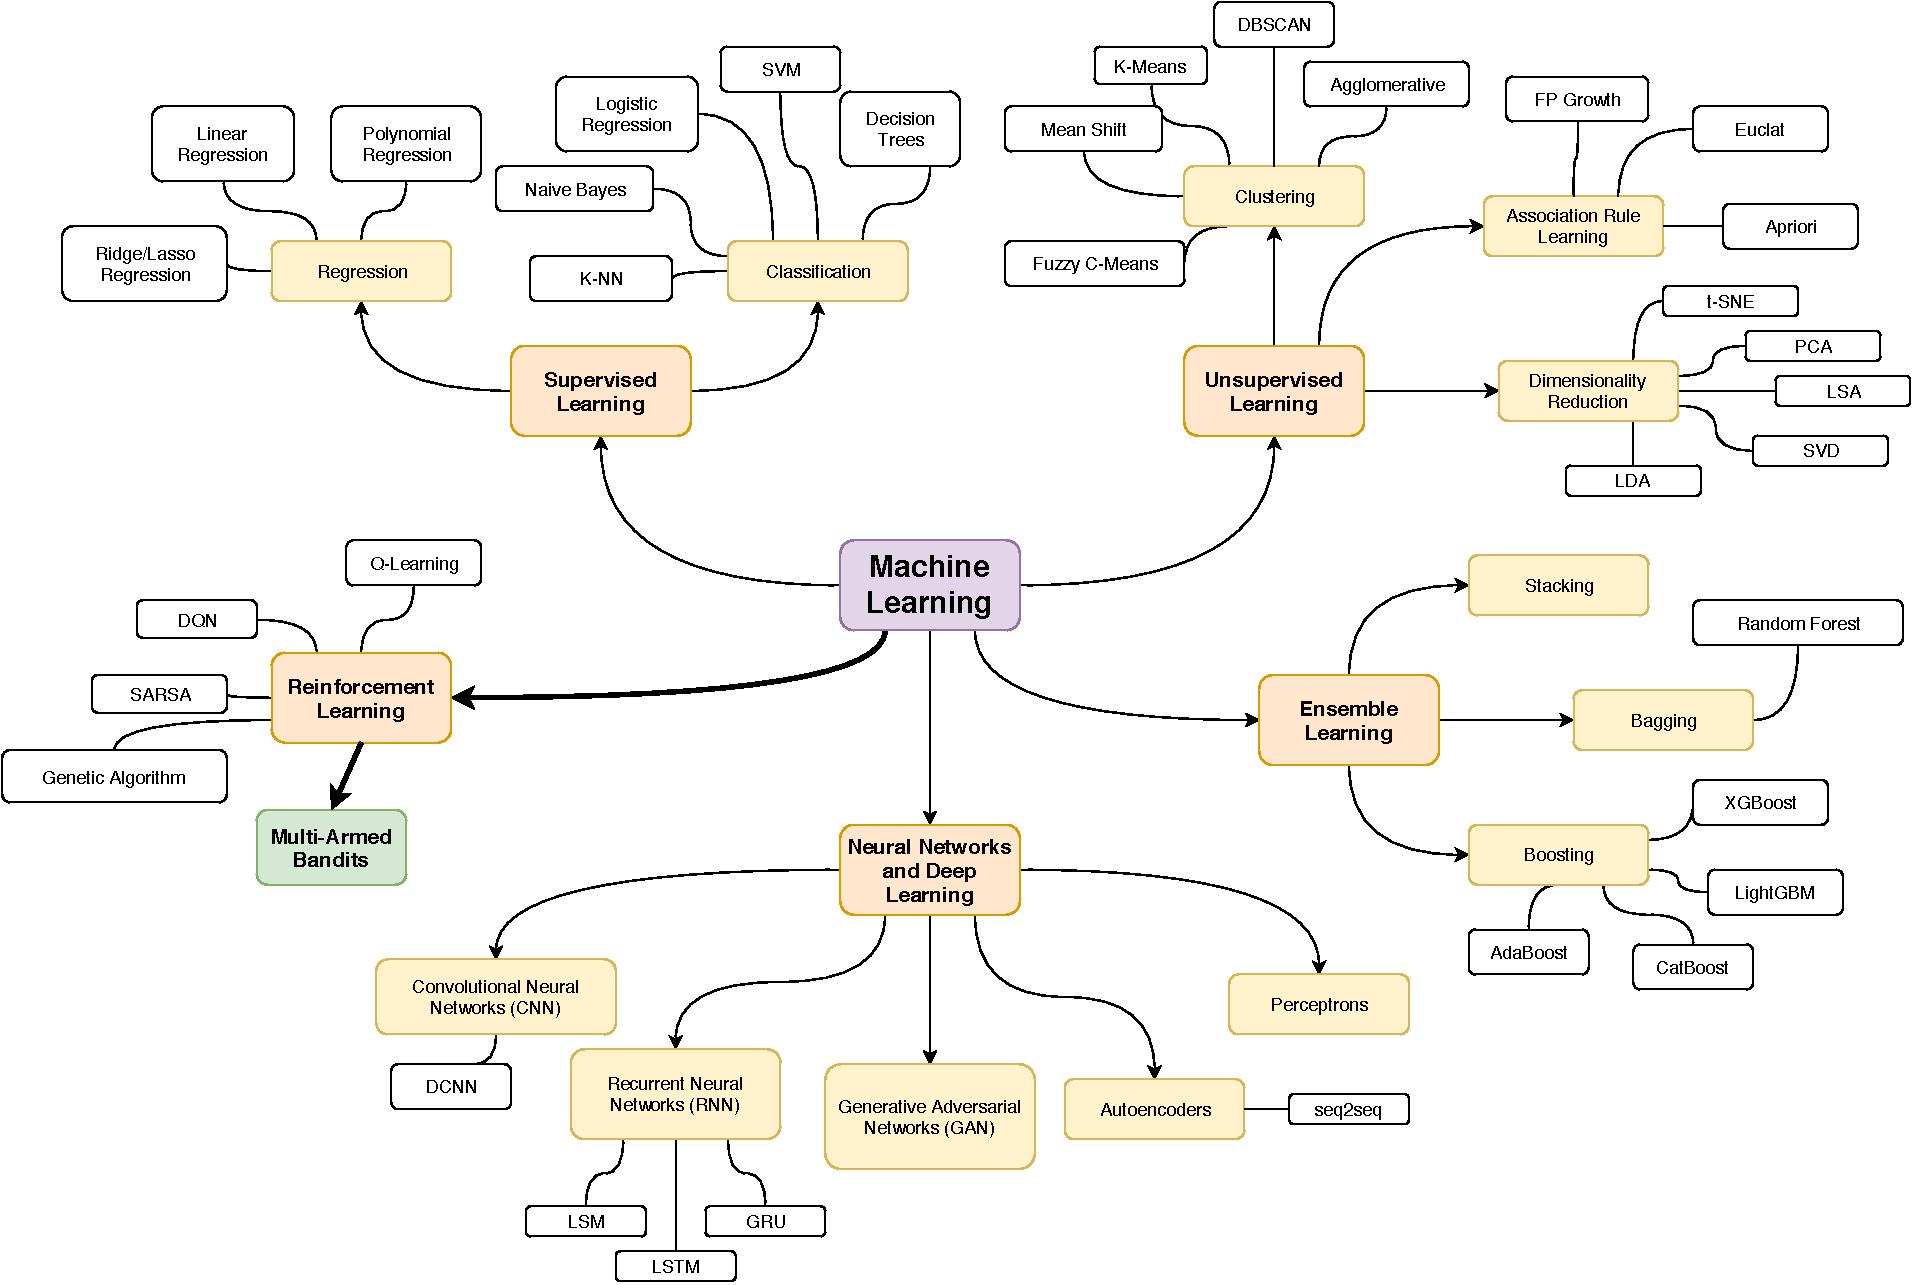
\includegraphics[width=0.95\textwidth]{machine-learning-map.pdf}
\caption{Classification of the main types of Machine Learning: MAB is a subset of Reinforcement Learning and RL is a subset of ML. MAB is RL with partial information, and RL is ML with no supervision or data, just an environment to interact with.}
\label{fig:1:MainTypesOfMachineLearning}
\end{figure}

We illustrate this idea of a \emph{learning cycle} alternating between actions and feedback,
in the following Figure~\ref{fig:1:ReinforcementLearningCycle}.
A player (or learner) interacts with its environment by taking an action $A(t)$ (\eg, a choice in a finite set, $A(t)\in\{1,\dots,K\}$, or a vector $A(t)\in\R^d$), and then observing a reward $r(t)$, which is a certain measure of success from the environment (\eg, $r(t)\in\{0,1\}$ for binary failure/success, or $r(t)\in\R$).
The goal of the player is to maximize its reward, by trials and errors (\ie,actions and rewards).
Many real-world problems can be framed as Reinforcement Learning problems, as illustrated by the survey \cite{bouneffouf2019survey} and Section~\ref{sec:2:applicationsofStochasticMAB}, for instance learning to walk or to drive, learning to play a board or computer game, or discovering which treatment is efficient in healing a certain disease (clinical trial).

% \begin{figure}[h!]
%     \centering
%     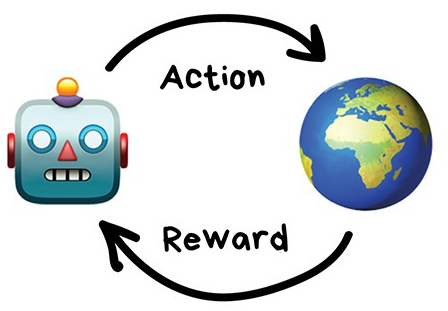
\includegraphics[width=0.25\textwidth]{Illustration_of_Reinforcement_Learning_action-reward_loop.png}
%     \caption{Reinforcement learning cycle, a learner interacts with its environment through actions, and observes a reward, iteratively. \copyright{} from \href{https://vas3k.com/blog/machine_learning/}{\texttt{VAS3k.com/blog/machine\_learning}}.}
%     \label{fig:1:ReinforcementLearningCycle}
% \end{figure}

\tikzstyle{block} = [align=center, draw, fill=gray!25, rectangle, minimum height=3em, minimum width=6em]
\begin{figure}[h!]
    \centering
    \resizebox{0.30\textwidth}{!}{
        \begin{tikzpicture}[auto,node distance=5cm,>=latex,scale=1.5]
            %
            % We start by placing the blocks
            \node [block] (player) at (0,0) {Player};
            % We draw an edge between the player and system block to
            \node [block] (environment) at (2,0) {Environment};
            % Once the nodes are placed, connecting them is easy.
            \draw [->] (player) to[bend left=90] node[pos=0.5] {Action} (environment);
            \draw [->] (environment) to[bend left=90] node[pos=0.5] {Reward} (player);
            %
        \end{tikzpicture}
    }
\caption{Reinforcement learning cycle: a learner interacts with its environment through actions, and observes a reward, iteratively.}
\label{fig:1:ReinforcementLearningCycle}
\end{figure}


% Il faut expliquer ce que c'est que les bandits, rapidement, et leur application à l'OSA
More precisely, in this thesis we focus on a certain kind of Reinforcement Learning models where the learning does not have access to the entire reaction of the environment after taking its action.
In other words, we focus on RL with limited feedback, when the player only sees the reward given by its action at every round, and not the reward that would have been given if she chose any other action.
This kind of limited feedback is called \emph{bandit information}, and we discuss the history and the concept of \emph{Multi-Armed Bandits} in details in the next Chapter~\ref{chapter:2}.
Clinical trials and treatment discovery was historically the first application of MAB, in $1933$ with the early work of W. Thompson \cite{Thompson33}.
%
Multi-Armed Bandits (MAB) are a simple yet powerful example of the well-known exploration/exploitation dilemma:
when facing a set of $K$ actions whose effects on the environment are unknown, a learning must balance between
exploration of the unknown actions, in order to collect more information about them,
and exploitation of the best action according to its current knowledge.


\paragraph{From IT to Cognitive Radio.}
%
Similarly, we can narrow down the second field of study of this thesis, steps by steps:
from Information Technologies (IT), to telecommunications, to wireless communications, then to Software Defined Radio (SDR),
and finally to Cognitive Radio (CR).
%
The transition from the historical approach of hardware-based radio to SDR architectures and is a gradual process that started in the early $1990$s and has accelerated in the $2000$s.
% https://en.wikipedia.org/wiki/Software-defined_radio
A SDR is a radio communication system where components that have been traditionally implemented in hardware (e.g. mixers, filters, amplifiers, modulators/demodulators, detectors, etc) are instead implemented by means of software on a personal computer or embedded system, with the exception of a unique pair of receiver/transmiter antennas.
Even though the SDR paradigm was initiated by the USA defense research, over the past years the industry has started to be interested by SDR, and CR have got significant attention from the academia and industry as well.
% CR has been the first answer to solve spectrum scarcity issue which collected a huge attention in early 21st century.
%
CR is not a standard technology, and as such it does not have a single definition, so let us start by quoting the definition of two researchers whose works were the roots of the development of CR, in the last $20$ years.
% - technologies de l'information > télécommunications > communications sans fil > radio intelligente > DSA > OSA
%
% je peux faire comme Navik, donner des définitions de la CR, citant d'autres travaux
\begin{itemize}
    \item
    Joseph Mittola in $1999$ said that
    \emph{``a really smart radio that would be self-, RF- and user-aware, and that would include software technology and machine learning capabilities along with a lot of high-fidelity knowledge of the radio environment''} \cite{Mitola99}.

    \item
    Then Simon Haykin in $2005$ also said that
    \emph{``a CR is an intelligent wireless communication system that is capable of being aware of its surroundings, learning, and adapting its operating parameters (\eg, transmit power and carrier frequency) on the fly with an objective of providing reliable anytime, anywhere, and spectrally efficient communication''} \cite{Haykin05}.
    He was the first to propose to use CR for dynamic spectrum access.

    \item
    The \href{https://en.wikipedia.org/wiki/Cognitive_radio}{Wikipedia encyclopedia} states
    \emph{``A cognitive radio (CR) is a radio that can be programmed and configured dynamically to use the best wireless channels in its vicinity to avoid user interference and congestion. Such a radio automatically detects available channels in wireless spectrum, then accordingly changes its transmission or reception parameters to allow more concurrent wireless communications in a given spectrum band at one location''}.
\end{itemize}


\TODOL{Je peux améliorer (ou enlever) ce passage qui site J.Toledano, ou alors le commenter en plus de détails ? J'aime bien son rapport en fait (j'aurai du le lire au début de ma thèse !)}
% https://www.economie.gouv.fr/files/files/PDF/french-spectrum-mission-executive-summary-2014-06-25.pdf
% https://www.economie.gouv.fr/files/files/PDF/rapport-gestion-dynamique-spectre-2014-06-30.pdf
The abstract of the ``Dynamic Spectrum Management For Innovation And Growth'' report by Joëlle Toledano, commissioned and published by the French government \cite{Toledano2014EnglishSummary,Toledano2014FrenchFull},
mentions different important problems:
%
\begin{itemize}\tightlist
    \item
    \emph{``In France, digital economy represents $5\%$ of GDP and affects $80\%$ of the French economy''}
    \item
    \emph{``Radio frequencies are essential to many sectors: communications, broadcasting, transportation, satellite networks, energy networks and smart grids, public or private security, defense, etc.''}
    %
    \item
    \emph{``Everyone agrees on the growing need for spectrum.
    This growing need results from two phenomena.
    On the one hand, mobile traffic should be multiplied by 13 to 25 fold between 2011 and 2017.
    On the other hand, the development of new innovative services such as the Internet of Things and its multiple applications (smart cities, e-health...), could lead to a growing number of connected devices, up to 50 billion in 2020, according to estimations.''}
    \item
    \emph{``Today, there are no more available frequencies in the easily exploitable frequency bands.
    Moreover, it is getting more and more difficult to resort to classical methods of frequency bands liberation.''}
    \item
    \emph{``Growing recourse to spectrum sharing, and in particular dynamic spectrum sharing, constitutes an important spectrum reserve.
    A particular sharing form, the use of unlicensed bands, open to all and free, has been intensely developed with the growth of Wi-Fi use.''}
\end{itemize}


\textbf{The spectrum scarcity issue.}
%
A major problem of current wireless technologies is the issue of spectrum scarcity:
in most kinds of frequency bands, the entire RF spectrum is now allocated and free bands no longer exist, limiting the possibility of adding new usage.
As illustrated in Figure~\ref{fig:1:United_States_Frequency_Allocations_Chart_2016_The_Radio_Spectrum} below, only a very small portion of the RF spectrum in the USA is not yet allocated, from $0$ to \SI{9}{\kilo\hertz}, while the rest of the displayed portion of the spectrum, from \SI{9}{\kilo\hertz} to \SI{300}{\giga\hertz}, is allocated to various usages, that goes from maritime radionavigation (historically the first usage of radio telecommunication) to space research, inter-satellite, mobile telephony and many other applications.
%
% Traditional regulatory structures have been built for an analog model and are not optimized for cognitive radio.
Regulatory bodies in the world, like the \href{https://www.fcc.gov/}{Federal Communications Commission} in the USA (see \href{https://www.fcc.gov/}{\texttt{FCC.gov}})
or \href{http://www.tdf.fr/}{TDF} in France (see \href{https://www.TDF.fr/}{\texttt{TDF.fr}}, previously known as \emph{``TéléDiffusion de France''}), as well as different independent measurement campaigns, found that most radio frequency spectrum was inefficiently utilized,
meaning that while a band can be allocated to a certain unique usage, it can be free from any user in certain times and/or places.
We refer to \cite{valenta2010survey} for a survey on spectrum utilization in Europe.

Cellular network bands are overloaded in most parts of the world, but other frequency bands (such as military, amateur radio and paging frequencies) are insufficiently utilized.
Independent studies performed in some countries confirmed that observation, and concluded that spectrum usage highly depends on time and place.
Moreover, the fixed spectrum allocation prevents rarely used frequencies, like those assigned to specific services, from being used, even when any unlicensed users would not cause noticeable interference to the assigned service.
Therefore, in the last $15$ years, regulatory bodies in the world have been considering whether to allow unlicensed users in licensed bands if they would not cause any interference to licensed users.
These initiatives have focused CR research on \textbf{Dynamic Spectrum Access (DSA)}.

\begin{figure}[h!]
    \centering
    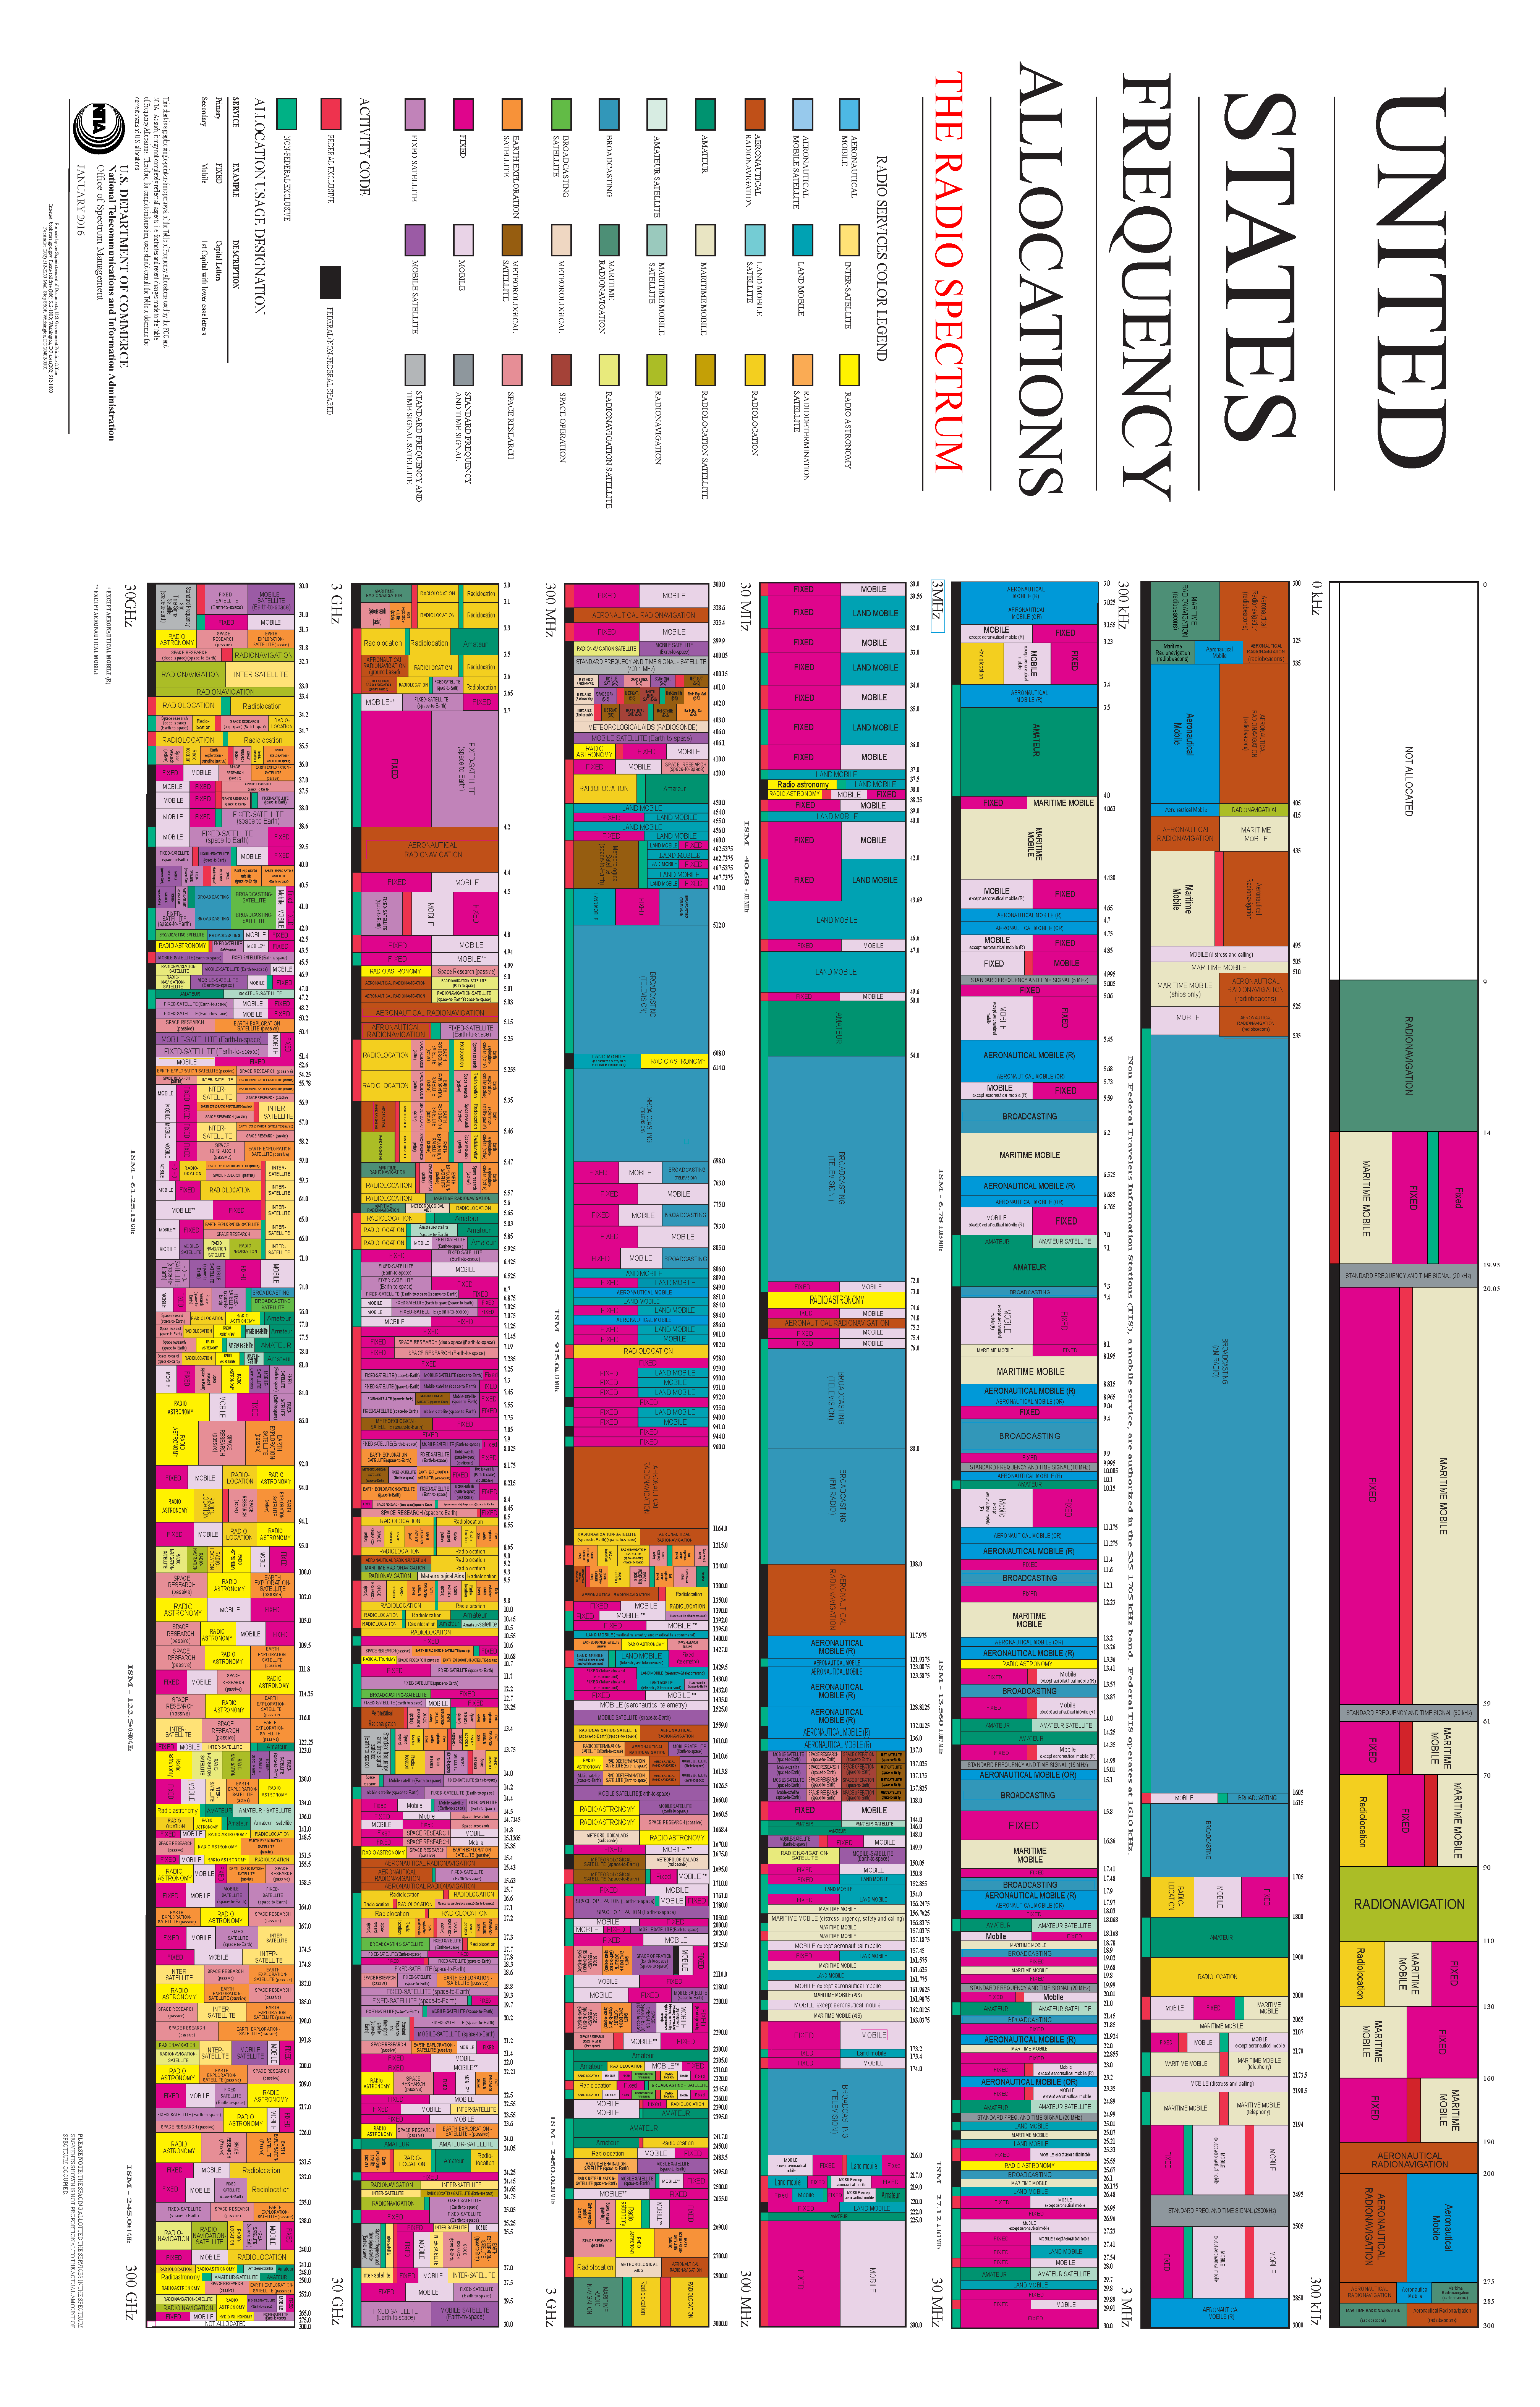
\includegraphics[width=0.65\textwidth,angle=90]{United_States_Frequency_Allocations_Chart_2016_The_Radio_Spectrum.pdf}
    \caption{A chart representing the allocation of radio spectrum in the USA in $2016$. Only a small share of the spectrum is not yet allocated, the top-left corner in white (it is in logarithmic scale from \SI{0}{\kilo\hertz} to \SI{300}{\giga\hertz}). \copyright{} Wikimedia.}
    % https://upload.wikimedia.org/wikipedia/commons/c/c7/United_States_Frequency_Allocations_Chart_2016_-_The_Radio_Spectrum.pdf?uselang=fr
    \label{fig:1:United_States_Frequency_Allocations_Chart_2016_The_Radio_Spectrum}
\end{figure}

% explain PU and SU in a few sentences
In licensed bands, there are Primary Users (PU) paying to access the network, for instance anybody has to pay to have a mobile phone number and use the mobile telephony network.
The PU have a strict priority over any other non-paying users, referred to as Secondary User (SU).
So even though the RF bands are allocated, real world measurements often show that some bands are not densely used, and thus if a SU is equipped with an efficient sensing capacity, it can analyze its environment, and use a licensed band if it is free of any PU.
% explain DSA
This defines the concept of DSA was thus proposed in the early $2000$s, and we refer to the survey \cite{Zhao07} for more details.
We focus on one example, the \textbf{Opportunistic Spectrum Access} (OSA) problem.


\paragraph{Opportunistic Spectrum Access.}
%
In OSA, the focus is on one SU accessing a licensed spectrum.
%
The following hypothesis are maid:
the SU is equipped with sensing,
and a consider a fixed and finite set of orthogonal channels, \ie, different frequency bands in a licensed spectrum.
For instance, it can be a set of three Wi-Fi channels at different frequency, emitted by the same Wi-Fi station.
Another hypothesis is that both PU and SU are synchronized in times, by sub-dividing the time in discrete time steps.
%
Thus if the SU spends a short time in the beginning of each time slot to do sensing, it can scan for the presence or absence of any PU before transmitting.
If a SU was able to sense for all the $K$ frequency bands, it could simply transmit in one of the free channels if any, or not transmit if all channels are used at a given time step.
However, sensing is known to be error-prone and costly, especially for wide-band sensing, thus most works on OSA limit the sensing capacity of SU to sensing only one channel at a time. This assumption, along with the regulation that PU cannot be disturbed, enforces the SU to transmit in the channel that it sensed.
% non negligible cost of radio reconfiguration

Focussing on one SU in an OSA network, it has to sequentially decide a channel to sense (in the set of $K\geq2$ channels), then it performs sensing, and finally it transmits in this channel if it is free.
The goal of the SU is to minimize its energy consumption (we remind that we focus on green radio) and to maximize its uplink data rate, or equivalently, to maximize its number of successful transmission.
%
If the different channels are not uniformly used by the PU, and if we assume a stationary hypothesis on the PU traffic, then the goal of the SU boils down to explore the different channels and exploiting the best ones.
This frames the Opportunistic Spectrum Access problem as a exploration/exploitation problem, white a finite set of actions (the channels, also called arms),
in a sequential action-then-feedback cycle (time steps are $t\in\N^*$),
under partial information feedback.
These three hypotheses are the ones that restrict from the general RL framework to the specific Multi-Armed Bandit case (see Figure~\ref{fig:1:ReinforcementLearningCycle}).


\paragraph{MAB for OSA, and a short presentation of the history of this research at the SCEE team.}
%
Previous works of our SCEE team showed that MAB can be used to model the OSA problem:
orthogonal frequency bands (or channels) are models by arms $k\in\{1,\dots,K\}$,
and the feedback obtained by the CR-equipped device after sensing the channel $k$ at time $t$ is modeled by a reward of $r(t) \in \{0,1\}$.
Indeed, $r(t) = 1$ indicates that no Primary User was sensed (and thus an uplink message can be sent), while a reward of $r(t)=0$ indicates that the channel $k$ is busy at time $t$ and no uplink message should be sent.
%
This model was first studied by Wassim Jouini during his PhD thesis with Christophe Moy, ten years ago, first with \cite{Jouini09} and later with \cite{Jouini10,Jouini12}.
His works were among the first ones to propose to use Reinforcement Learning for Cognitive Radio and the OSA problem, especially the MAB model and the \UCB{} algorithm,
along the early works of Qing Zhao and her team, for instance with the works \cite{Liu08,Zhao10}.
%
Shortly after in $2014$, proof-of-concepts using real-world radio hardware and Software Defined Radio were developed by Christophe Moy and his student Clément Robert \cite{RobertSDR2014,MoyWSR2014}.

In a second PhD thesis supervised by Christophe Moy \cite{Modi17PhD} from $2014$ to $2017$, Navikkumar Modi studied the impact of using MAB algorithms to optimize channel selection on the battery life of a wireless device.
On the one hand, running a MAB algorithm such as UCB-like algorithms was proven to be useful and can bring significant improvement in terms of successful transmission rates, directly increasing the battery life of the device.
On the other hand, classical MAB algorithms tend to switch arms a lot of times, especially in the beginning of the learning process, and this induces a lot of dynamical hardware reconfiguration for the wireless device, as selecting a different channel requires a change in the radio hardware used by the device.
Each hardware reconfiguration costs energy for the device, and quickly switching algorithms will lead to a reduction of the battery life.
The tradeoff between the two aspects is studied empirically in
\cite{modiDemo2016}.
%
In $2017$, Christophe Moy continued to work on this direction, with a post-doctoral student, Sumit J. Darak, leading to the following publications
\cite{darak2016bayesian,Darak16,modiDemo2016,kumar2016two}.
%
For example, proof-of-concepts like \cite{kumar2016two} have proven the capability of such approaches on real radio signals for OSA,
%
Some analysis on real radio measurements made for HF ionospheric channels have also proven that solutions based on MAB learning is appropriate and solves efficiently this kind of decision-making problems on real-world wireless signals \cite{Melian15}.
%
Since $2017$, Sumit J. Darak and his team at IIIT Delhi have been very active in the research on cognitive radio using multi-armed bandits, and some of their recent works are illustrated with real-world demo using USRP and the MATLAB/Simulink system
\cite{KumarYadav2018,SawantKumar2018,JoshiKumar2018}.

\TODOL{Raccourcir toutes les fois où je parle des travaux sur l'OSA après dans la suite de la thèse !}


\paragraph{Limitations and specifities of IoT networks.}
%
The aforementioned previous works have shown that MAB algorithms can be applied with success for the OSA problem.
But if we consider CR-ready devices that cannot perform sensing, such as low-cost and low energy consumption end-devices designed for the future Internet of Things networks, the MAB model that uses sensing to detect PU in the OSA case can no longer be applied.
Moreover, in most cases, the IoT networks use unlicensed bands, and as such there are no longer a distinction between PU and SU.
%
The specificities of IoT networks can be listed as follows.
\begin{itemize}
    \item
    most IoT networks run in unlicensed bands (no more distinction between PU and SU),
    \item
    most IoT devices are very low-cost devices, with low material and computational capacities,
    meaning that they are not equipped with any sensing capabilities,
    \item
    a single IoT base station will have to handle a very large number of devices,
    and cannot send coordination orders to them in order to optimize the network,
    \item
    IoT devices have low duty cycles (only a few messages every minute) to very low duty cycles (only a few messages a day).
    % FIXME more specificities?
\end{itemize}

One could think that in the absence of sensing, Reinforcement Learning is no longer possible, but any real IoT device still receives some information about its environment after some or every transmissions.
In most IoT standards an up-link message sent to a base station is usually followed by a down-link message sent back by the base station, to indicate if the up-link message was successfully received and understood.
%
By using this feedback, that consists in an \emph{acknowledgement} (\Ack) message received shortly after every successful transmission, or in an absence of \Ack{} avery a failed transmission, it is possible that an IoT end-device can also use RL algorithms to optimize its communications.
%
To the best of our knowledge, this direction of research has never been studied before the year $2016$ and the beginning of this PhD.

% \newpage % WARNING

% ----------------------------------------------------------------------------
\section{Our contributions}
\label{sec:1:contributions}

We start by formulating the problem studied in this thesis, and then we develop our approach.

\paragraph{Problematic.}
%
If we sum-up the studied problems and summarize them in one question, it would be the following:
\emph{``Can we adapt the decision making tools already successfully applied to Cognitve Radio for Opportunistic Spectrum Access to the specific needs of CR for the future IoT networks ?''}
%
We answer partially to this problematic by the following research steps.

\paragraph{Focusing on MAB algorithms.}
% FIXME
%
We started by exploring the rich literature of multi-armed bandits,
as many different algorithms exist, with lots of variants on the simple problem presented above (see \cite{LattimoreBanditAlgorithmsBook,Slivkins2019} for surveys).
We thus start the first Part~\ref{part:Introduction} of this thesis with Chapter~\ref{chapter:2}, which presents the MAB model and gives a review of the most important algorithms designed to solve stochastic and stationary MAB problems.
%
In order to clearly understand which algorithms could be applied to the aforementioned problems of CR and IoT,
we were not only interested by the usual measure of performance of any MAB algorithm (its regret, see below in Section~\ref{sec:2:lowerUpperBoundsRegret}),
but also by their empirical performances in terms of computational complexity and storage requirements, both from the point of view of the theoretical analyses and real-world measurements on time and memory footprints of the different algorithms.

Our exploration of the large number of MAB algorithms and models developed in the recent literature
has gave us the ambition to write a single piece of software were we could easily implement new models and algorithms, in order to compare the existing ones and empirically explores the performances of newly proposed algorithms.
To answer this goal, we produced a Python library of simulation of MAB problems.
%
We wrote the most exhaustive open-source simulation library for MAB problems, called SMPyBandits, which is published online under an open-source licence \cite{SMPyBandits,SMPyBanditsJMLR}.
We present in details its architecture and its features in Chapter~\ref{chapter:3}, along with different examples of its usage.
A full documentation is available online, as well as exhaustive instructions to reproduce the experiments used in the rest of this thesis.

Because there are so many different MAB algorithms, we are also interested by the question of how practitioner can chose the one she will implement in a given IoT object.
To answer this question, we present two approaches.
The first one is an empirical comparison of the most efficient and well-known existing algorithms in Section~\ref{sec:3:reviewSPAlgorithms} and \ref{sec:3:timeAndMemoryCosts}, where it appears that simple algorithms such as \UCB{} \cite{Auer02}, Thompson sampling \cite{Thompson33} and \klUCB{} \cite{KLUCBJournal} are the most efficient in terms of regret, and offer a good balance between regret and (time and memory) complexity.
The second approach is an online algorithm selection, consisting in aggregating a set of algorithms and automatically discovering which one performs the most efficiently, against a given problem, with our contribution \Aggr{} that we detail in Chapter~\ref{chapter:25}.


\paragraph{Focusing on IoT networks.}
%
\TODOL{Je dois faire ça d'ici mercredi matin}

First model \cite{Bonnefoi17}, CROWNCOM paper, model to detail

We already explained in Chapter~\ref{chapter:1} that
unlicensed bands are more and more used and considered for mobile and LAN communication standards (WiFi, LTE-U), and for Internet of Things (IoT) standards for short-range (ZigBee, Z-Wave, Bluetooth) and long-range (LoRaWAN, SIGFOX, Ingenu, Weightless) communications \cite{Centenaro16}.
This heavy use of unlicensed bands, in particular with the expected exponential growth of the number of IoT devices, will cause performance drop, due to radio collisions that could even compromise IoT promises.

Efficient Medium Access (MAC) policies allow devices to avoid interfering traffic and can significantly reduce the spectrum contention problem in unlicensed bands.
As end-devices battery life is a key constraint of IoT networks,
and as IoT networks are decentralized (\ie, the devices initiate transmissions),
this leads to IoT protocols using as low signaling overhead as possible and simple ALOHA-based mechanisms.
%
In this chapter, we analyze the performance of Multi-Armed Bandits (MAB) algorithms, that could be used in combination with a time-frequency slotted ALOHA-based protocol.
Even without changing anything of the level of IoT standards, our proposal is just an add-on capability that can be used on a unit-per-unit basis.
We consider the Upper-Confidence Bound (\UCB) \cite{Auer02}, and the Thompson-Sampling (TS) algorithms \cite{Thompson33,AgrawalGoyal11,
Kaufmann12Thompson}, for the first model. For the demonstration as well as for the second model, without loss of generality, we preferred to focus on heuristics based on the simplest algorithm (\ie, \UCB), to give a clear presentation of the different ideas explored to solve the problem of learning in order to retransmit efficiently.

The aim of this section is to assess the potential gain of learning algorithms in IoT scenarios, even when the number of intelligent devices in the network increases,
and the network usage is more and more fluctuating.
% and the stochastic hypothesis is more and more violated.
To do that, we suppose an IoT network made of two types of devices: \emph{static devices} that use only one channel (fixed in time), and \emph{dynamic devices} that can choose the channel for each of their transmissions. Static devices form an interfering traffic, which could be generated by devices using other standards as well.
Note that instead of assuming that each static device uses a fixed channel, we could also assume a looser hypothesis: if each static device uses a fixed sub-set of the $K$ channels, and a purely uniform random access in its set of considered channels, then \emph{in average} the observed occupancy of the $K$ channels can be modeled as if it were occupied by (more) static devices using only one channel. So our first hypothesis is actually not constraining.
We first evaluate the probability of collision if dynamic devices randomly select channels (that is, a naive approach), and if a centralized controller would optimally distribute all of them in the channels at the beginning of the scenario.
This second approach is ideal, but not realistic the most common situation of decentralized co-located IoT networks, and it is just used here as a reference.
Then, these three reference scenarios allow to evaluate the performance of bandit algorithms, such as \UCB{} and TS, in a decentralized network, in terms of successful communication rate, as it reflects the network efficiency.
We show that these algorithms have near-optimal performance, even when the proportion of end-devices increases and the interfering traffic from other devices becomes less and less stochastic.

Verify this first model empirically: proof of concept \cite{Besson2018ICT}
\TODOL{Je dois faire ça d'ici mercredi matin}

Second model with decision making also for the retransmissions of packets \cite{Bonnefoi2019WCNC}
\TODOL{Je dois faire ça d'ici mercredi matin}

Selfish
\TODOL{Je dois faire ça d'ici mercredi matin}

Understand Selfish in the simpler framework of multi-player MAB
\TODOL{Je dois faire ça d'ici mercredi matin}

In the OSA setting, we failed
\TODOL{Je dois faire ça d'ici mercredi matin}

But we proposed new algorithms for this problem, and relaunched the research on this model \cite{Besson2018ALT}
\TODOL{Je dois faire ça d'ici mercredi matin}



\paragraph{Our approach.}
%
Our approach for the aforementioned problems is summarized as follows:
we propose a couple of new models of decision making for IoT networks, on the device's side, for the spectrum access problem.
By considering the difference between the hypothesis of previously studied models for the OSA problem and our problem at end for IoT, we identify the constraints and specificities of applying decentralized ML for IoT devices.
%
Like for the OSA, we can apply successfully model the decision making problem as a Multi-Armed Bandit problem.
We showed on numerical simulations as well as on a real-world proof-of-concept that applying low-cost sequential learning algorithms coming from the MAB literature successfully reduce the collision rate of IoT end-devices.
We proposed new algorithms, some of which are proven to converge efficiently.

\TODOL{Je dois faire ça d'ici mercredi matin}

% %
% directions de recherches

% - réfléchir aux modèles, quelles hypothèses sont retirées comparé au modèle OSA

% - analyser mathématiquement les modèles

% - proposer des solutions : algorithmes, dont la convergence est justifiée, ou heuristiques

% - des simulations logicielles

% - des démonstrations matérielles

% - et en bonus on obtient aussi de belles contributions théoriques



% FIXME c'est bon tout ce qu'on a avant ?

\TODOL{Je suis content de la suite de l'intro : aperçu des contributions, plans de thèse, liste des publications}

\newpage % WARNING

% ----------------------------------------------------------------------------
\paragraph{Summary of the contributions}
\label{sec:1:summaryOfContributions}

To summarize the main contributions of this thesis, we can list the following points:

\begin{itemize}
    % \item
    % We present the concepts and the notations of the multi-armed bandit problem in Chapter~\ref{chapter:2}, from a mathematical point-of-view.
    % But we also follow a didactic approach as we use an online interactive demonstration designed to let anyone play against a small bandit problem from his/her browser, in Section~\ref{par:2:interactiveDemoDiscoverMAB}.

    % \item
    % We give a short literature review of stochastic bandit algorithms in Section~\ref{sec:2:famousMABalgorithms}.

    \item
    We wrote the most exhaustive open-source simulation library for MAB problems, called SMPyBandits, which is published online under an open-source licence \cite{SMPyBandits,SMPyBanditsJMLR}.
    We present in details its architecture and its features in Chapter~\ref{chapter:3}, along with different examples of its usage.
    A full documentation is available online, as well as exhaustive instructions to reproduce the experiments used in the rest of this thesis.

    \item
    % We present the problem of choosing which algorithm a practitioner should use, or algorithm selection from the rich collection of different MAB available, in Section~\ref{sec:2:chooseYourPreferredBanditAlgorithm}.
    We present in Chapter~\ref{chapter:25} an algorithm called \Aggr{} for aggregation of algorithms as an online solution to the algorithm selection problem, and numerical simulations to illustrate that it achieves state-of-the-art empirical performances
    \cite{Besson2018WCNC}.
    % with \textbf{Aggregator} (WCNC 2018)

    \item
    We propose different models for IoT networks, in Chapter~\ref{chapter:4}, where end-devices with cognitive radio capabilities can implement MAB algorithms on their side, to automatically increase their battery life and allow more devices to use the same network while maintaining a high Quality of Service
    \cite{Bonnefoi17,Besson2019WCNC,Bonnefoi2019WCNC}.
    % (CROWNCOM 2017, ICT demo 2018, WCNC 2019 and MOTIoN 2019)

    \item
    We implemented a proof-of-concept of the aforementioned model \cite{Besson2018ICT}, and we present it in details in Section~\ref{sec:4:gnuradio}. We made a video showcasing our demonstration, hosted at \texttt{\href{https://youtu.be/HospLNQhcMk}{youtu.be/HospLNQhcMk}}.

    % \item
    % The source code for the two previously mentioned contributions are all published online, along with clear instructions for reproducing our work.

    \item
    We formalize the multi-players bandit model, and we introduced three variants, in Chapter~\ref{chapter:5}.
    For the case with sensing information, we propose two new algorithms, and we give an analysis for our algorithm \MCTopM{} to show it is order-optimal,
    as well as extensive numerical experiments to demonstrate its good performance in comparison with the rest of the literature.
    Our work \cite{Besson2018ALT} also gave a new impulse on research on multi-players bandits, as some recent research works built up on our results.

    % \item
    % We also give a detailed literature review of the different extensions of the multi-players MAB model, which we believe was never written before.
    % % were  (ALT 2018, and 4-8 works inspired by our article since then). State-of-the-art with our algorithm MCTopM + klUCB for multi-players bandits "with sensing", empirical state-of-the-art with our simple (but wrong) "selfish" approach in case of "no sensing"

    \item
    We also present the piece-wise stationary MAB model, in Chapter~\ref{chapter:6}, and a detailed literature review of the research on non stationary MAB \cite{Besson2019GLRT,Besson2019Gretsi}.
    Following two recent works, we propose a new actively adaptive algorithm for the piece-wise stationary problem, \GLRklUCB, that achieves state-of-the-art performance.
    % - Literature review on non stationary models and algorithms, state-of-the-art for piece-wise stationary with our algorithm, GLR test + klUCB

    \item
    The last contribution of this thesis is a literature review of the possible use cases of the sequentially doubling horizon trick technique for MAB problems,
    and a unified and more generic analysis of two families of doubling tricks.
    This lead to the article \cite{Besson2018DoublingTricks}, which is quickly presented in Appendix~\ref{app:2:DoublingTricks}.
\end{itemize}


% ----------------------------------------------------------------------------
\section{Organization of the thesis}
\label{sec:1:organization}

The reading order of the manuscript can be any top-down path between the Introduction in the current Chapter~\ref{chapter:1}, and the Conclusion in the last Chapter~\ref{chapter:conclusion}. As the graph in Figure~\ref{fig:1:organization} shows,
the thesis is organized in two parts.

\begin{figure}[h!]
    \centering
    \resizebox{0.95\textwidth}{!}{
    \begin{tikzpicture}[>=latex',line join=bevel,scale=2.25]
        %
        \node[align=center] (introduction) at (0,3.25) [rectangle,draw,fill=blue!10] {\textbf{Chapter~\ref{chapter:1}}\\Introduction};
        \node[align=center] (chapter2) at (0,2.25) [rectangle,draw,fill=red!10] {\textbf{Chapter~\ref{chapter:2}}\\Stochastic and Stationary\\Multi-Armed Bandit models};
        \node[align=center] (chapter3) at (-2.5,2.25) [rectangle,draw,fill=red!10] {\textbf{Chapter~\ref{chapter:3}}\\SMPyBandits: simulation\\library for MAB};
        \node[align=center] (chapter25) at (+2.5,2.25) [rectangle,draw,fill=red!10] {\textbf{Chapter~\ref{chapter:25}}\\Online selection\\of the best algorithm};
        \node[align=center] (chapter4) at (-2.5,1) [rectangle,draw,fill=green!10] {\textbf{Chapter~\ref{chapter:4}}\\Two MAB models\\for IoT networks};
        \node[align=center] (chapter5) at (0,1) [rectangle,draw,fill=green!10] {\textbf{Chapter~\ref{chapter:5}}\\Multi-players\\Multi-Armed Bandits};
        \node[align=center] (chapter6) at (2.5,1) [rectangle,draw,fill=green!10] {\textbf{Chapter~\ref{chapter:6}}\\Non-stationary\\Multi-Armed Bandits};
        \node[align=center] (conclusion) at (0,-0.25) [rectangle,draw,fill=blue!10] {\textbf{Chapter~\ref{chapter:conclusion}}\\General Conclusion};
        \node[align=center] (appendix) at (2.5,-0.25) [rectangle,draw,fill=blue!10] {Appendix};
        %
        \draw [color=black,thick,->] (introduction) to (chapter2);
        \draw [color=black,thick,<->] (chapter2) to (chapter3);
        \draw [color=black,thick,<->] (chapter2) to (chapter25);
        \draw [color=black,thick,->] (chapter2) to (chapter4);
        \draw [color=black,thick,->] (chapter2) to (chapter5);
        \draw [color=black,densely dotted,<->]   (chapter4) to (chapter5);
        % \draw [color=black,densely dotted,->] -| (chapter3) to (chapter25);
        % \draw [color=black,densely dotted,->] -| (chapter25) to (chapter6);
        \draw [color=black,densely dotted,<->]   (chapter5) to (chapter6);
        \draw [color=black,thick,->] (chapter2) to (chapter6);
        \draw [color=black,thick,->] (chapter4) to (conclusion);
        \draw [color=black,thick,->] (chapter5) to (conclusion);
        \draw [color=black,thick,->] (chapter6) to (conclusion);
        \draw [color=black,thick,->] (conclusion) to (appendix);
        %
    \end{tikzpicture}
    }
    \caption[Organization of the thesis: a reading map]{A reading map of the thesis. Any top-down path containing Chapter~\ref{chapter:1}, Chapter~\ref{chapter:2}, at least one of the three Chapters~\ref{chapter:4}, \ref{chapter:5} and \ref{chapter:6}, and the Conclusion is a self contained way to read this thesis.}
    \label{fig:1:organization}
\end{figure}

% \begin{itemize}
    % \item
In Part~\ref{part:Introduction}, we start by the next Chapter~\ref{chapter:2}, required for the rest of the document as we introduce the MAB models, the concepts and the notations used in this thesis.
Conversely, even if Chapters~\ref{chapter:2}, \ref{chapter:5} and \ref{chapter:6} use numerical simulations based on our simulation library SMPyBandits, the Chapter~\ref{chapter:3} where we present it is not required to understand them.
We conclude this part with Chapter~\ref{chapter:25}, which is also not mandatory for the rest of this thesis, and which details one of the first contributions of this thesis, a new algorithm for online MAB algorithms selection.

    % \item
Then the second Part~\ref{part:MABIOT} contain three chapters, that are included in both the logical and chronological orders, but can be read almost independently.
Chapter~\ref{chapter:4} starts by presenting different models of IoT networks where MAB algorithms have been used with success. Our two models are interesting and close to reality, but they appeared to be too general to propose a mathematical analysis of the good empirical performance of the considered solutions.
For this reason, we weaken the models for the rest of the document,
and both Chapters~\ref{chapter:5} and \ref{chapter:6} studies an intermediate model, lying between the stationary single-player MAB model from Chapter~\ref{chapter:2} and the IoT networks models from Chapter~\ref{chapter:4}.
% \end{itemize}


% WARNING
\newpage


% ----------------------------------------------------------------------------
\section{List of publications}
\label{sec:1:listPublications}

We conclude this chapter with a list of works published during this PhD.
All the following works are published entirely and freely, on the HAL platform (see the \href{https://hal.archives-ouvertes.fr/}{\texttt{HAL.Archives-Ouvertes.fr}} website).
The complete list can be found on
\href{https://cv.archives-ouvertes.fr/lilian-besson/}{\texttt{CV.Archives-Ouvertes.fr/lilian-besson}}.


% =============================================================================
\subsection*{Publications in international conferences with proceedings}

\begin{itemize}
\item
    \emph{Decentralized Spectrum Learning for IoT Wireless Networks Collision Mitigation},
    by Christophe Moy \& \textbf{Lilian Besson}.
    1st International ISIoT workshop,
    % \footnote{~See \href{https://sites.google.com/view/ISIoT2019}{\texttt{sites.google.com/view/ISIoT2019}}},
    at \emph{Conference on Distributed Computing in Sensor Systems},
    % \footnote{~IEEE DCOSS 2019, see \href{http://2019.dcoss.org}{\texttt{2019.dcoss.org}}},
    Santorini, Greece, May 2019.
    % \href{https://HAL.Inria.fr/hal-02144465}{\texttt{HAL.Inria.fr/hal-02144465}}.
    See Section~\ref{sec:4:gnuradio}.
    \cite{MoyBesson2019}

\item
    \emph{Upper-Confidence Bound for Channel Selection in LPWA Networks with Retransmissions},
    by Rémi Bonnefoi, \textbf{Lilian Besson}, J. Manco-Vasquez \& Christophe Moy.
    1st International MOTIoN workshop,
    % \footnote{~MOTIoN 2019, see \href{https://sites.google.com/view/wcncworkshop-motion2019}{\texttt{sites.google.com/view/wcncworkshop-motion2019}}},
    at \emph{IEEE WCNC}, Marrakech, Morocco, April 2019.
    % \href{https://HAL.Inria.fr/hal-02049824}{\texttt{HAL.Inria.fr/hal-02049824}}.
    See Section~\ref{sec:4:retransmissions}.
    \cite{Bonnefoi2019WCNC}

\item
    \emph{GNU Radio Implementation of MALIN: ``Multi-Armed bandits Learning for Internet-of-things Networks''},
    by \textbf{Lilian Besson}, Rémi Bonnefoi \& Christophe Moy.
    \emph{Wireless Communication and Networks Conference},
    % \footnote{~IEEE WCNC 2019, see \href{http://wcnc2019.ieee-wcnc.org}{\texttt{wcnc2019.ieee-wcnc.org}}},
    Marrakech, Morocco, April 2019,
    % \href{https://HAL.Inria.fr/hal-02006825}{\texttt{HAL.Inria.fr/hal-02006825}}.
    See Section~\ref{sec:4:gnuradio}.
    \cite{Besson2019WCNC}

\item
    \emph{Multi-Player Bandits Revisited},
    by \textbf{Lilian Besson} \& Emilie Kaufmann.
    \emph{Algorithmic Learning Theory},
    % \footnote{~ALT 2018, see \href{http://www.cs.cornell.edu/conferences/alt2018}{\texttt{www.cs.cornell.edu/conferences/alt2018}}},
    Lanzarote, Spain, April 2018,
    % \href{https://HAL.Inria.fr/hal-01629733}{\texttt{HAL.Inria.fr/hal-01629733}}.
    See Chapter~\ref{chapter:5}.
    \cite{Besson2018ALT}

\item
    \emph{Aggregation of Multi-Armed Bandits learning algorithms for Opportunistic Spectrum Access},
    by \textbf{Lilian Besson}, Emilie Kaufmann \& Christophe Moy.
    \emph{Wireless Communication and Networks Conference},
    % \footnote{~IEEE WCNC 2018, see \href{http://wcnc2018.ieee-wcnc.org}{\texttt{wcnc2018.ieee-wcnc.org}}},
    Barcelona, Spain, April 2018,
    % \href{https://HAL.Inria.fr/hal-01705292}{\texttt{HAL.Inria.fr/hal-01705292}}.
    See Chapter~\ref{chapter:25}.
    \cite{Besson2018WCNC}

\item
    \emph{Multi-Armed Bandit Learning in IoT Networks and non-stationary settings},
    by Rémi Bonnefoi, \textbf{Lilian Besson}, Christophe Moy, Emilie Kaufmann \& J. Palicot.
    \emph{Conference on Cognitive Radio Oriented Wireless Networks},
    % \footnote{~CROWNCOM 2017, see \href{http://crowncom.org/2017}{\texttt{crowncom.org/2017}}},
    Lisboa, Portugal, Septembre $2017$,
    % \href{https://HAL.Inria.fr/hal-01575419}{\texttt{HAL.Inria.fr/hal-01575419}},
    \textbf{Best Paper Award}.
    See Section~\ref{sec:4:firstModel}.
    \cite{Bonnefoi17}

\end{itemize}

% =============================================================================
\subsection*{Demonstration in international conferences}

\begin{itemize}

\item
    \emph{MALIN: ``Multi-Arm bandit Learning for Iot Networks'' with GRC: A TestBed Implementation and Demonstration that Learning Helps},
    by \textbf{Lilian Besson}, Rémi Bonnefoi, Christophe Moy.
    Demonstration presented at \emph{International Conference on Communication},
    % \footnote{~ICT 2018, see \href{http://ict-2018.org/demos}{\texttt{ict-2018.org/demos}}},
    Saint-Malo, France in June $2018$.
    See \href{https://YouTu.be/HospLNQhcMk}{\texttt{YouTu.be/HospLNQhcMk}} for a $6$-minutes presentation video.
    See Section~\ref{sec:4:gnuradio}.
    \cite{Besson2018ICT}

\end{itemize}


% =============================================================================
\subsection*{French language conference with proceedings}
% \textbf{Submitted works}

\begin{itemize}
\item
    \emph{Analyse non asymptotique d'un test séquentiel de détection de ruptures et application aux bandits non stationnaires} (in French),
    by \textbf{Lilian Besson} \& Emilie Kaufmann,
    GRETSI 2019,
    % \footnote{~GRETSI 2019, see \href{http://GRETSI.fr/colloque2019}{\texttt{GRETSI.fr/colloque2019}}},
    August $2019$,
    % \href{https://HAL.Inria.fr/hal-02006471}{\texttt{HAL.Inria.fr/hal-02006471}}.
    See Chapter~\ref{chapter:6}.
    \cite{Besson2019Gretsi}

\end{itemize}


% =============================================================================
\subsection*{In progress works waiting for a new submission}

\begin{itemize}

\item
    \emph{The Generalized Likelihood Ratio Test meets klUCB: an Improved Algorithm for Piece-Wise Non-Stationary Bandits},
    by \textbf{Lilian Besson} \& Emilie Kaufmann,
    February $2019$.
    See Chapter~\ref{chapter:6}.
    Preprint at \href{https://HAL.Inria.fr/hal-02006471}{\texttt{HAL.Inria.fr/hal-02006471}}.
    \cite{Besson2019GLRT}

\item
    \emph{SMPyBandits: an Open-Source Research Framework for Single and Multi-Players Multi-Arms Bandits (MAB) Algorithms in Python},
    by \textbf{Lilian Besson}, active development between October $2016$ and March $2019$,
    \href{https://HAL.Inria.fr/hal-01840022}{\texttt{HAL.Inria.fr/hal-01840022}}.
    It currently consists in about $40000$ lines of code, hosted on \href{https://GitHub.com/SMPyBandits}{\texttt{GitHub.com/SMPyBandits}},
    and a complete documentation on \href{https://SMPyBandits.rtfd.io}{\texttt{SMPyBandits.rtfd.io}} and \href{https://SMPyBandits.GitHub.io}{\texttt{SMPyBandits.GitHub.io}}.
    See Chapter~\ref{chapter:3}.
    \cite{SMPyBandits,SMPyBanditsJMLR}

\item
    \emph{What Doubling-Trick Can and Can't Do for Multi-Armed Bandits},
    by \textbf{Lilian Besson} \& Emilie Kaufmann,
    September $2018$.
    See Appendix~\ref{app:2:DoublingTricks}.
    Preprint at \href{https://HAL.Inria.fr/hal-01736357}{\texttt{HAL.Inria.fr/hal-01736357}}.
    \cite{Besson2018DoublingTricks}

\end{itemize}


% % =============================================================================
% \textbf{Other works}

% \begin{itemize}
% \item
%     \emph{A Note on the Ei Function and a Useful Sum-Inequality},
%     by \textbf{Lilian Besson},
%     February $2018$,
%     \href{https://HAL.Inria.fr/hal-01847480}{\texttt{HAL.Inria.fr/hal-01847480}}.

% \end{itemize}


% % =============================================================================
% \textbf{Presentations in seminars and conferences}

% \textbf{Seminars.}
%     I gave some presentations in the following events:
%     SequeL team seminar at Inria Lille in September and December $2017$, and June $2019$;
%     SCEE team seminar at CentraleSupélec, Rennes campus, in October $2017$, February $2018$ and June $2019$;
%     as well as
%     for the GDR ISIS day held in Issy-les-Moulineaux on November $2017$,
%     for the brown-bag seminar at ENSAI in Bruz in January $2018$,
%     for the weekly seminar at CMAP lab at École Polytechnique in October $2018$,
%     for the weekly seminar of the PANAMA project-team at IRISA / Inria Rennes in June $2019$.

% \textbf{Tutorial.}
%     I gave a tutorial on the Julia language, at IETR seminar in Vannes in June $2018$,
%     with Pierre Haessig (see \href{https://pierreh.eu/}{\texttt{pierreh.eu}}), see \href{https://HAL.Inria.fr/cel-01830248}{\texttt{HAL.Inria.fr/cel-01830248}}.

% \textbf{Training.}
%     I was also in charge of ``GouTP'' training sessions for about $30$ PhD students at CentraleSupélec Rennes.
%     We had a lot of various $1$h training sessions between January $2017$ and June $2019$,
%     and I gave about $12$ training sessions, on various topics including Python, \texttt{git}, HAL and arXiv, the Julia language and Bib\TeX{}.


% % =============================================================================
% \textbf{Other experiences}

% \textbf{Conferences.}
%     I attended the following conferences:
% 	\emph{International Conference on Communication} ICC (Paris), May $2017$,
%     \emph{Conference on Learning Theory} COLT (Amsterdam), July $2017$,
%     \emph{Conference on Cognitive Radio Oriented Wireless Networks} CROWNCOM (Lisboa), September $2017$,
%     \emph{Conference on Algorithmic Learning Theory} ALT (Lanzarote), April $2018$,
%     \emph{Wireless Communication and Networking Conference} WCNC (Barcelona), April $2018$,
% 	\emph{International Conference on Telecommunication} ICT (Saint-Malo), June $2018$,
%     \emph{Wireless Communication and Networking Conference} WCNC (Marrakech), April $2019$,
%     \emph{Colloque francophone de traitement du signal et des images} GRETSI (Lille), August $2019$.

% \textbf{Seminars.}
%     I attended the following seminars:
% 	\emph{Workshop Learn with Earning} (Rotterdam), May $2018$,
% 	\emph{Workshop on Optimization and Learning} (Toulouse), September $2018$,
% 	\emph{European Workshop on Reinforcement Learning} (Lille), October $2018$.

% \textbf{Responsibilities.}
%     I was the president of the PhD Students Association of IETR lab (ADDI, \texttt{addi.asso.insa-rennes.fr}) in $2017$.
%     I was notably in charge of organizing the PhD Students day at Rennes, in June $2017$, with about $350$ people, and presentation of a research poster\footnote{~See \href{https://HAL.Inria.fr/hal-02013839}{\texttt{HAL.Inria.fr/hal-02013839}}}
%     I also helped for the organization and presented another poster\footnote{~See \href{https://HAL.Inria.fr/hal-02013847}{\texttt{HAL.Inria.fr/hal-02013847}}} at the ``IETR : Interagir Évaluer Transmettre Réunir'' seminar, held in Vannes in June $2018$.

% \textbf{Reviews.}
% 	for \emph{European Workshop on Reinforcement Learning}\footnote{~EWRL 2018, see \href{https://ewrl.wordpress.com/ewrl14-2018}{\texttt{ewrl.wordpress.com/ewrl14-2018}}} (Lille), in October $2018$, I reviewed $5$ papers.
% 	I helped colleagues for articles submitted at international conferences \emph{AISTATS} $2019$, \emph{NeurIPS} $2017$ et $2018$, and \emph{COLT} $2018$ and $2019$, for about 10 \emph{reviews}.

% \textbf{System Administrator.}
% 	maintaining our workstations running GNU/Linux and Windows
% 	at SCEE team,
% 	and our cognitive radio test-bed using USRP cards and the GNU Radio software,
% 	from January $2017$ to September $2018$.

% WARNING
\vfill{}

\paragraph{Copyright notice.}
%
This document and the additional resources required to compile it (including \LaTeX{} code, Python snippets, images etc)
are \href{https://github.com/Naereen/phd-thesis/}{publicly published},
under the terms of the open-source \href{https://lbesson.mit-license.org/}{\emph{MIT License}},
online at \href{https://github.com/Naereen/phd-thesis/}{\texttt{GitHub.com/Naereen/phd-thesis/}}.

% FIXME
% \TODOL{Open source the repository as soon as I defended my thesis!}

\begin{center}
    \textbf{Copyright 2016-2019, \copyright ~Lilian~Besson.}
\end{center}
